% Native editable composition of three verified, unchanged debugger captures.
\begin{figure}[htbp]
\centering
\sbox0{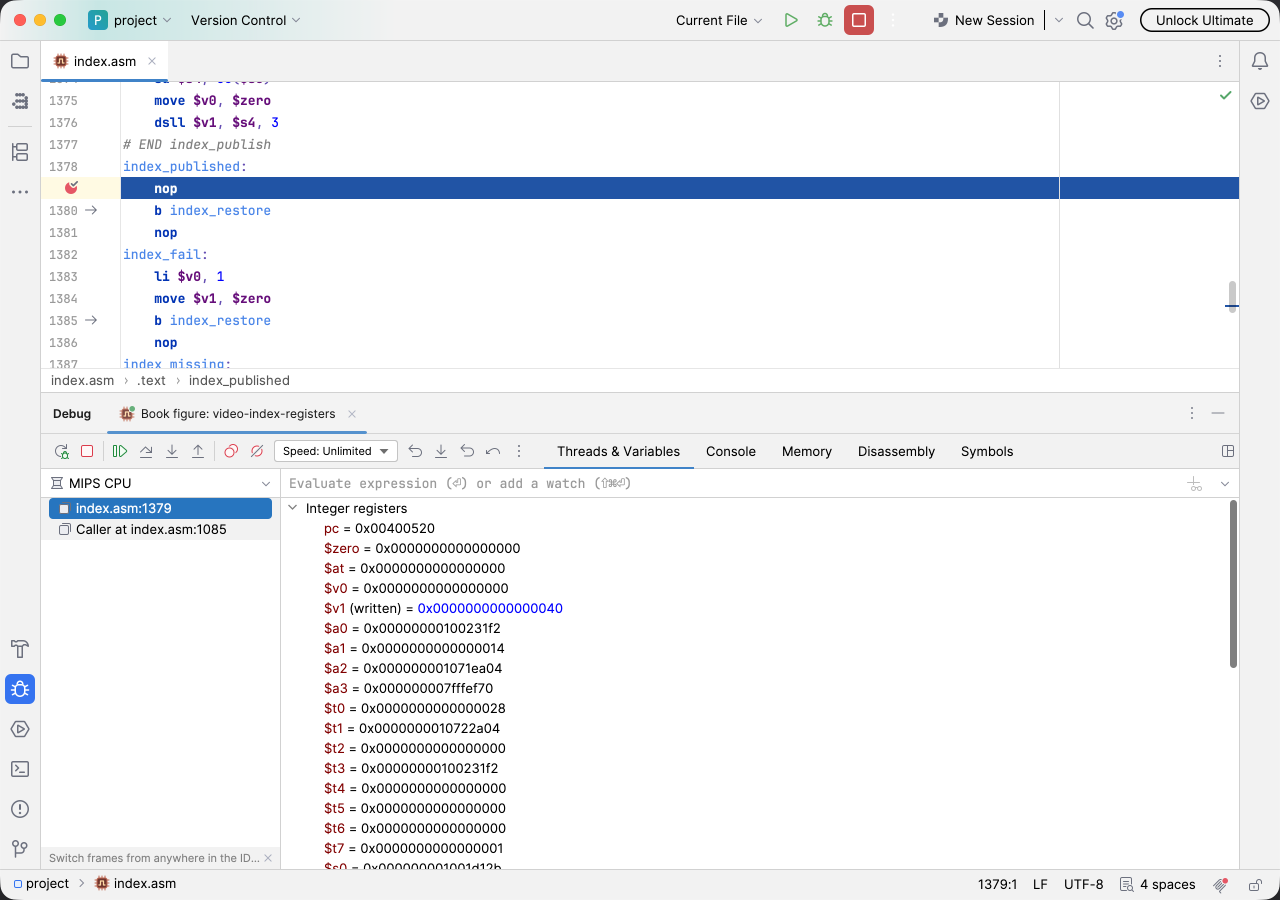
\includegraphics[artifact]{book/captures/034-lossless-video/video-index-publication/registers.png}}
\sbox2{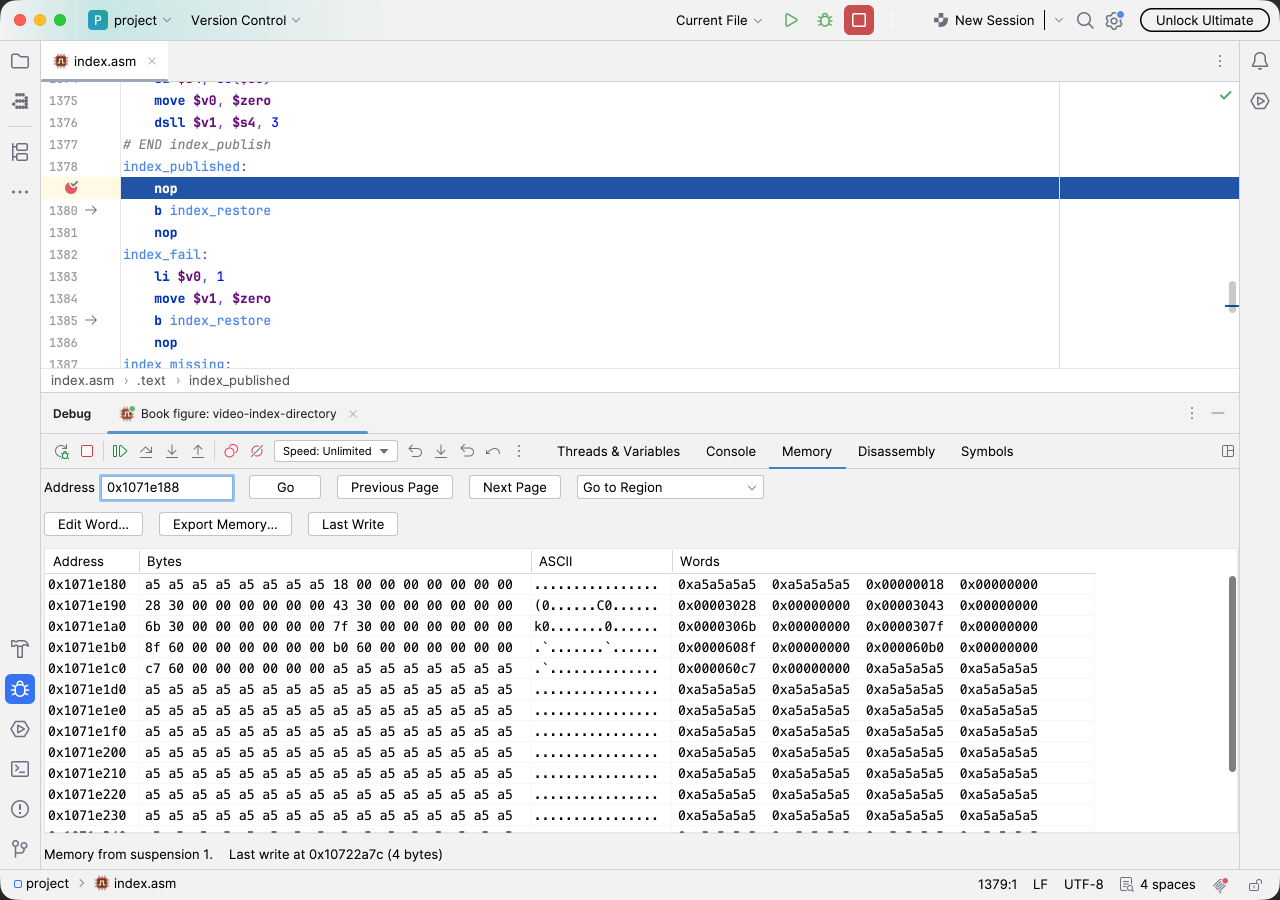
\includegraphics[artifact]{book/captures/034-lossless-video/video-index-publication/directory.png}}
\sbox4{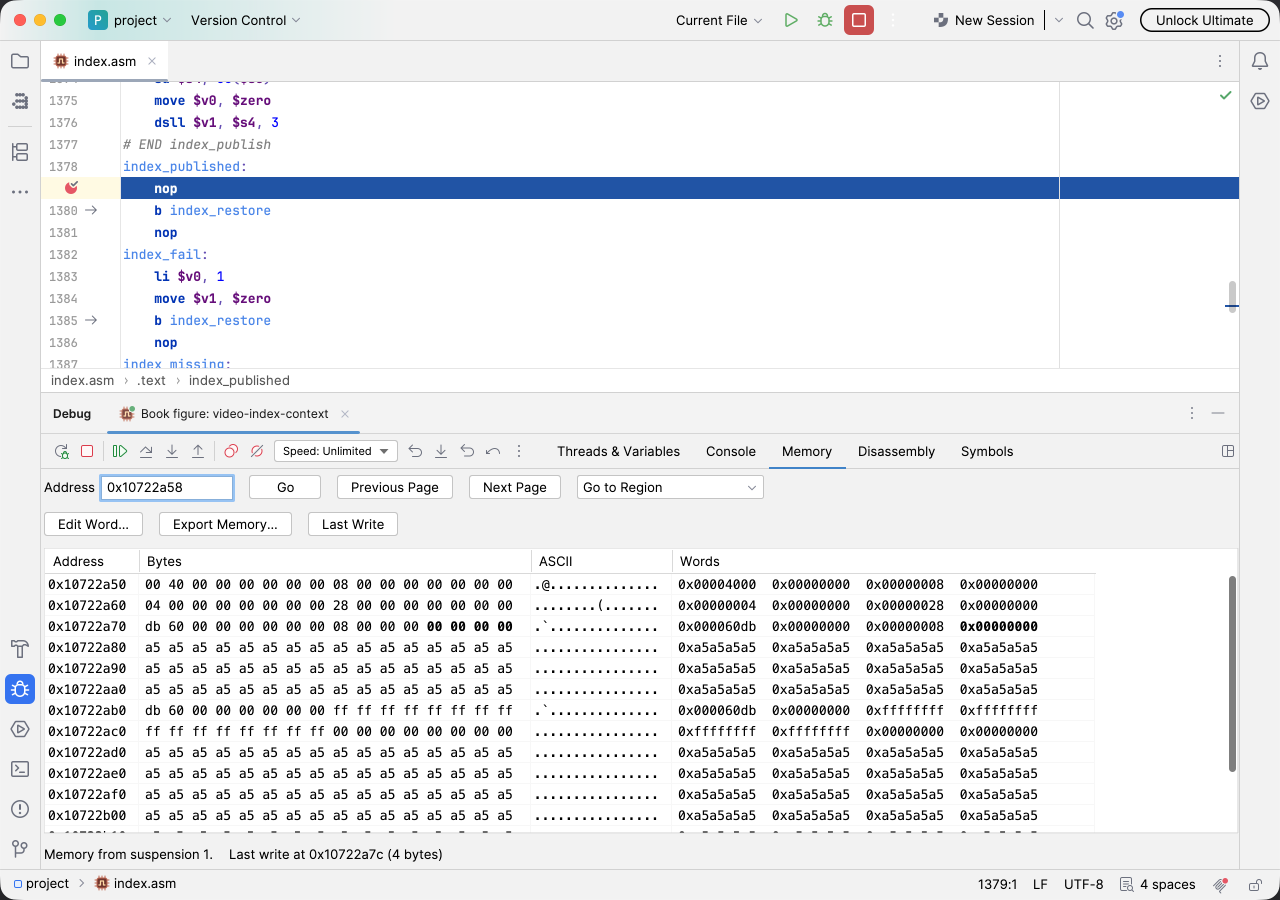
\includegraphics[artifact]{book/captures/034-lossless-video/video-index-publication/context.png}}
\edef\MARSindexsourceLeft{\the\dimexpr0.036718750\wd0\relax}
\edef\MARSindexsourceBottom{\the\dimexpr0.776666667\ht0\relax}
\edef\MARSindexsourceRight{\the\dimexpr0.611718750\wd0\relax}
\edef\MARSindexsourceTop{\the\dimexpr0.170000000\ht0\relax}
\edef\MARSindexdirectoryLeft{\the\dimexpr0.520312500\wd2\relax}
\edef\MARSindexdirectoryBottom{\the\dimexpr0.245555556\ht2\relax}
\edef\MARSindexdirectoryRight{\the\dimexpr0.139843750\wd2\relax}
\edef\MARSindexdirectoryTop{\the\dimexpr0.611111111\ht2\relax}
\edef\MARSindexcontextLeft{\the\dimexpr0.520312500\wd4\relax}
\edef\MARSindexcontextBottom{\the\dimexpr0.292222222\ht4\relax}
\edef\MARSindexcontextRight{\the\dimexpr0.139843750\wd4\relax}
\edef\MARSindexcontextTop{\the\dimexpr0.611111111\ht4\relax}
\edef\MARSindexreturnsLeft{\the\dimexpr0.246093750\wd0\relax}
\edef\MARSindexreturnsBottom{\the\dimexpr0.313333333\ht0\relax}
\edef\MARSindexreturnsRight{\the\dimexpr0.553906250\wd0\relax}
\edef\MARSindexreturnsTop{\the\dimexpr0.642222222\ht0\relax}
\begin{tikzpicture}[alt={Four annotated debugger details at index_published, before its nop. Detail 1 marks the next instruction. In this little-endian run each 64-bit memory value appears as its low 32-bit word followed by its high word. Detail 2 shows eight directory offsets in decimal: 24, 12328, 12355, 12395, 12415, 24719, 24752, 24775. Two leading and two trailing A5-pattern words are retained outside the active entries. Detail 3 begins with retained scratch capacity 16384, then published frame count 8, period 4, duration 40 milliseconds, file bytes 24795 and directory entries 8. Detail 4 shows v0 equal to zero and v1 equal to 64 bytes.}]
\node[anchor=north west,inner sep=0,font=\small\bfseries] (source-title) at (6mm,0) {Paused publication checkpoint};
\node[anchor=north west,inner sep=0] (source) at ([yshift=-2mm]source-title.south west) {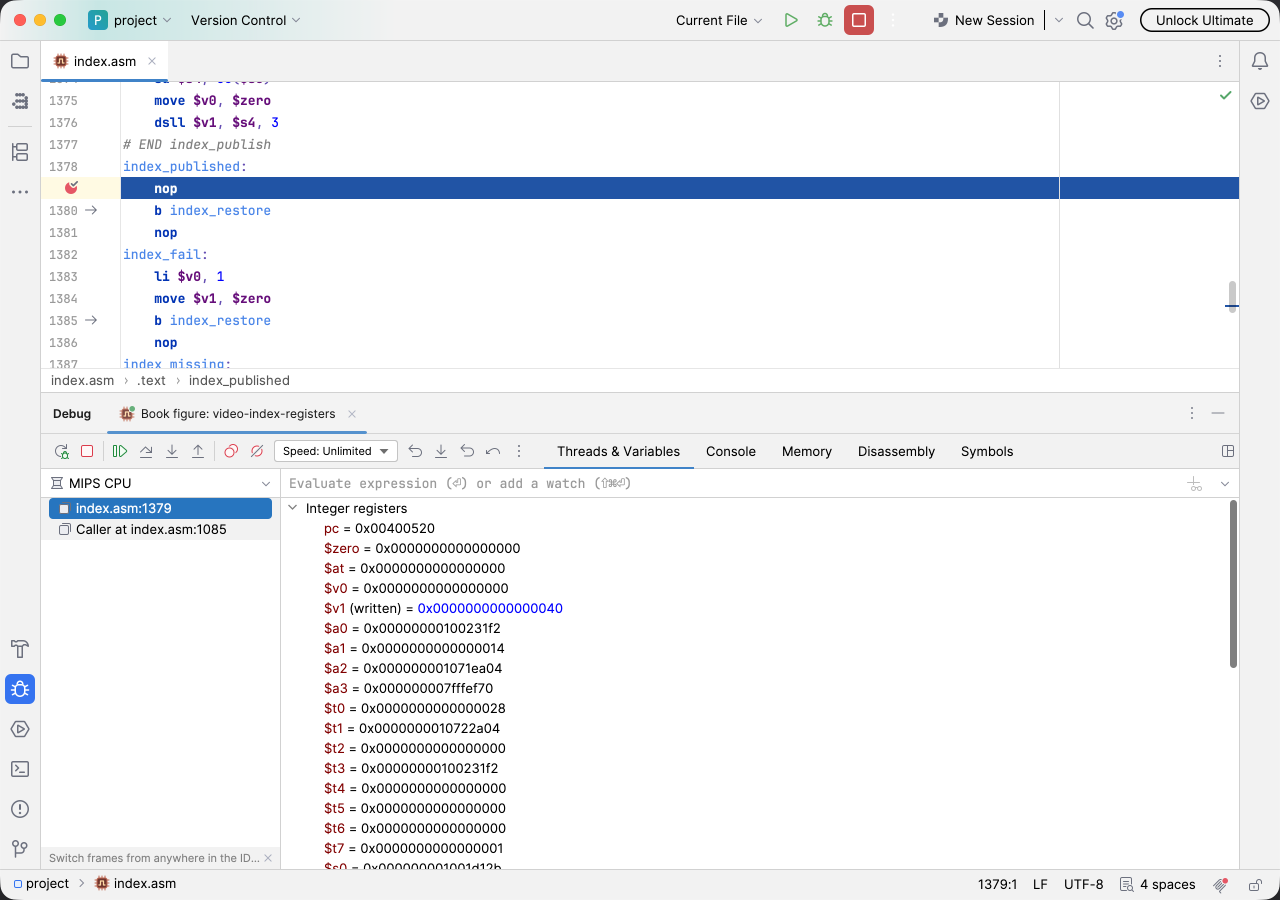
\includegraphics[width=0.68\linewidth,artifact,trim={\MARSindexsourceLeft{} \MARSindexsourceBottom{} \MARSindexsourceRight{} \MARSindexsourceTop{}},clip]{book/captures/034-lossless-video/video-index-publication/registers.png}};
\begin{scope}[shift={(source.south west)},x={($(source.south east)-(source.south west)$)},y={($(source.north west)-(source.south west)$)}]
\draw[black,line width=0.7pt] (0.168888889,0.041666667) rectangle (0.288888889,0.500000000);
\node[draw=black,fill=white,circle,inner sep=1.5pt,font=\footnotesize] at ($(0.168888889,0.500000000)+(-3mm,0)$) {1};
\end{scope}
\node[anchor=north west,inner sep=0,font=\small\bfseries] (directory-title) at ([yshift=-4mm]source.south west) {Directory offsets in the native Words column};
\node[anchor=north west,inner sep=0] (directory) at ([yshift=-2mm]directory-title.south west) {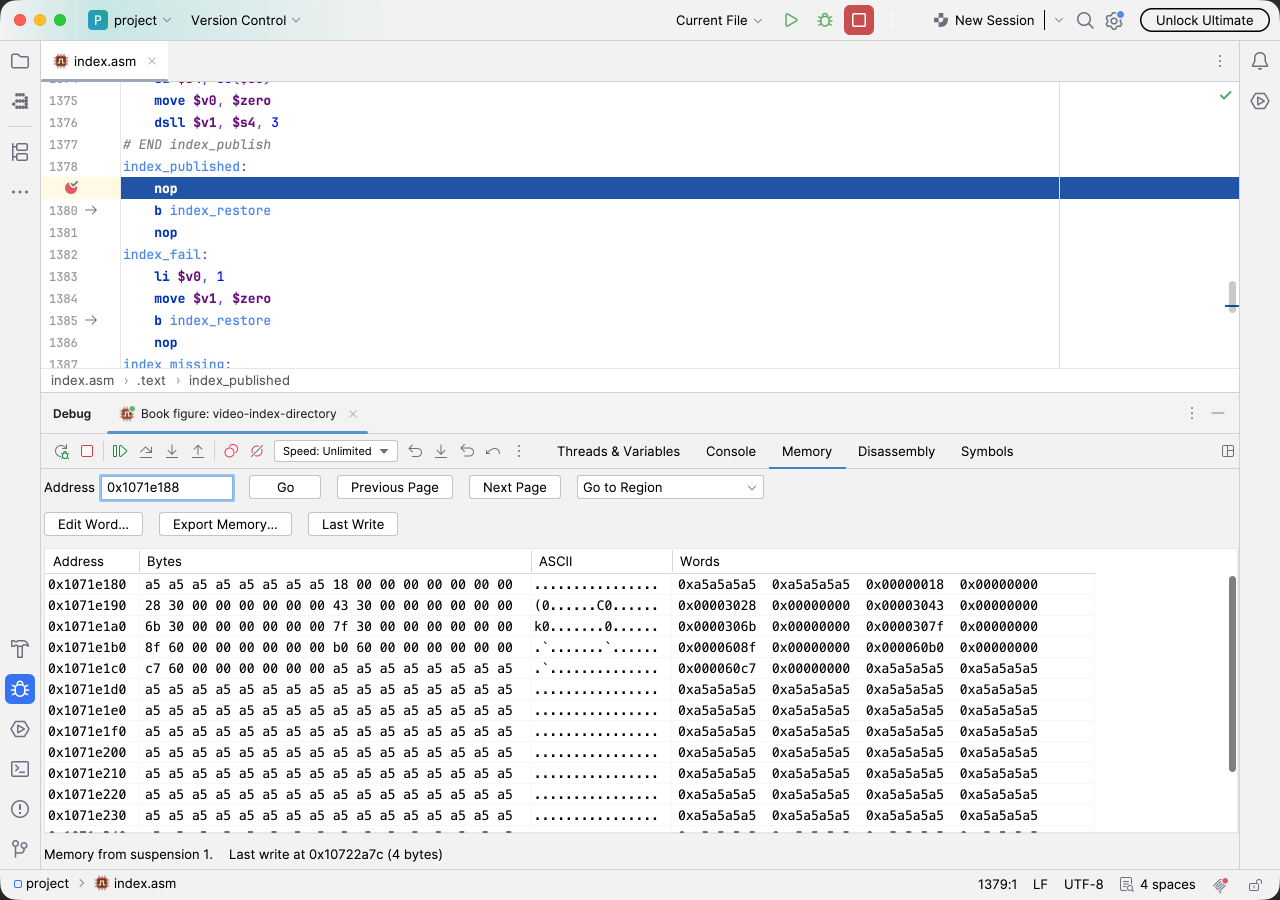
\includegraphics[width=0.86\linewidth,artifact,trim={\MARSindexdirectoryLeft{} \MARSindexdirectoryBottom{} \MARSindexdirectoryRight{} \MARSindexdirectoryTop{}},clip]{book/captures/034-lossless-video/video-index-publication/directory.png}};
\begin{scope}[shift={(directory.south west)},x={($(directory.south east)-(directory.south west)$)},y={($(directory.north west)-(directory.south west)$)}]
\draw[black,line width=0.7pt] (0.013793103,0.000000000) rectangle (0.986206897,0.813953488);
\node[draw=black,fill=white,circle,inner sep=1.5pt,font=\footnotesize] at ($(0.013793103,0.813953488)+(-3mm,0)$) {2};
\end{scope}
\node[anchor=north west,inner sep=0,font=\small\bfseries] (context-title) at ([yshift=-4mm]directory.south west) {Retained and published context fields};
\node[anchor=north west,inner sep=0] (context) at ([yshift=-2mm]context-title.south west) {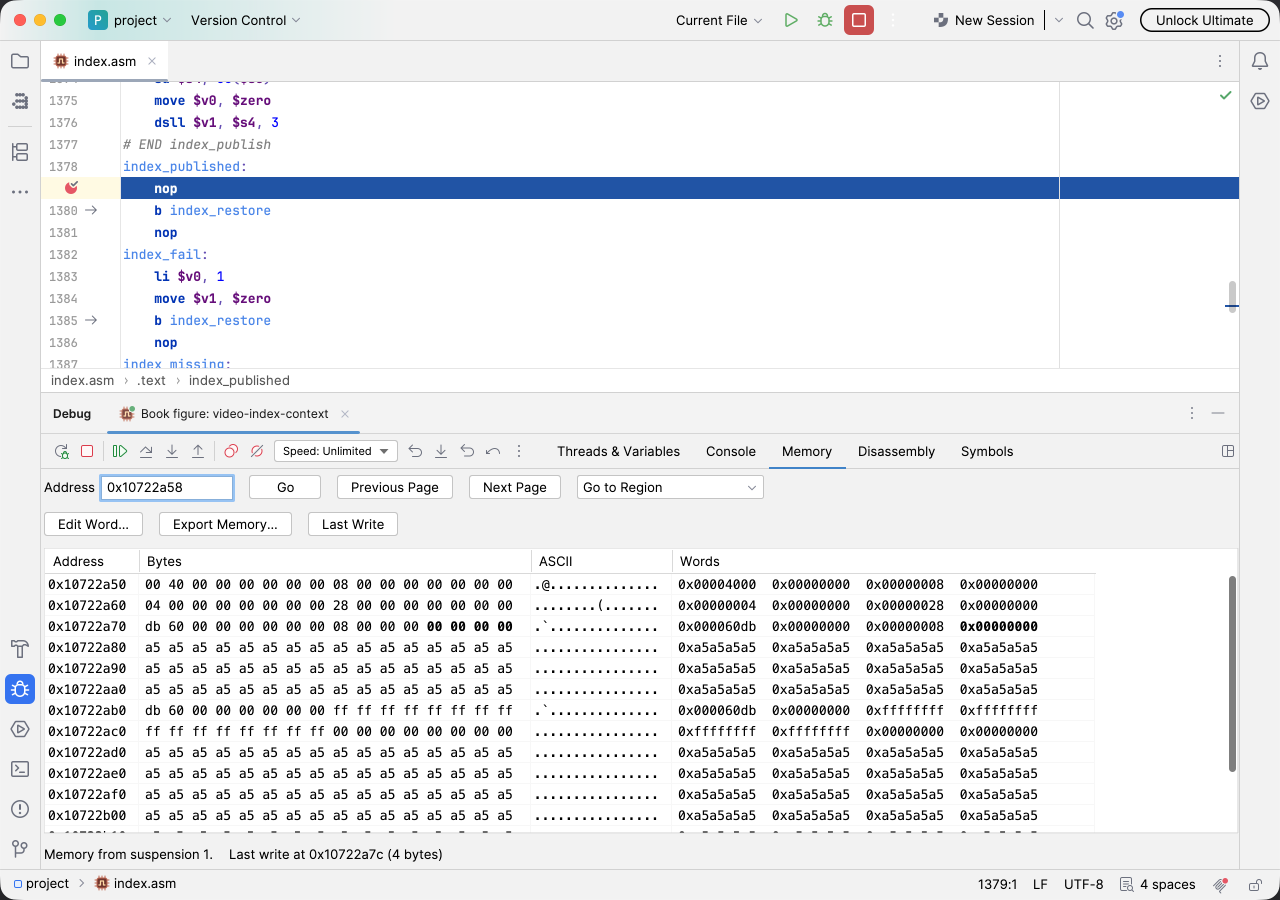
\includegraphics[width=0.86\linewidth,artifact,trim={\MARSindexcontextLeft{} \MARSindexcontextBottom{} \MARSindexcontextRight{} \MARSindexcontextTop{}},clip]{book/captures/034-lossless-video/video-index-publication/context.png}};
\begin{scope}[shift={(context.south west)},x={($(context.south east)-(context.south west)$)},y={($(context.north west)-(context.south west)$)}]
\draw[black,line width=0.7pt] (0.013793103,0.000000000) rectangle (0.986206897,0.724137931);
\node[draw=black,fill=white,circle,inner sep=1.5pt,font=\footnotesize] at ($(0.013793103,0.724137931)+(-3mm,0)$) {3};
\end{scope}
\node[anchor=north west,inner sep=0,font=\small\bfseries] (returns-title) at ([yshift=-4mm]context.south west) {Success and the active directory size};
\node[anchor=north west,inner sep=0] (returns) at ([yshift=-2mm]returns-title.south west) {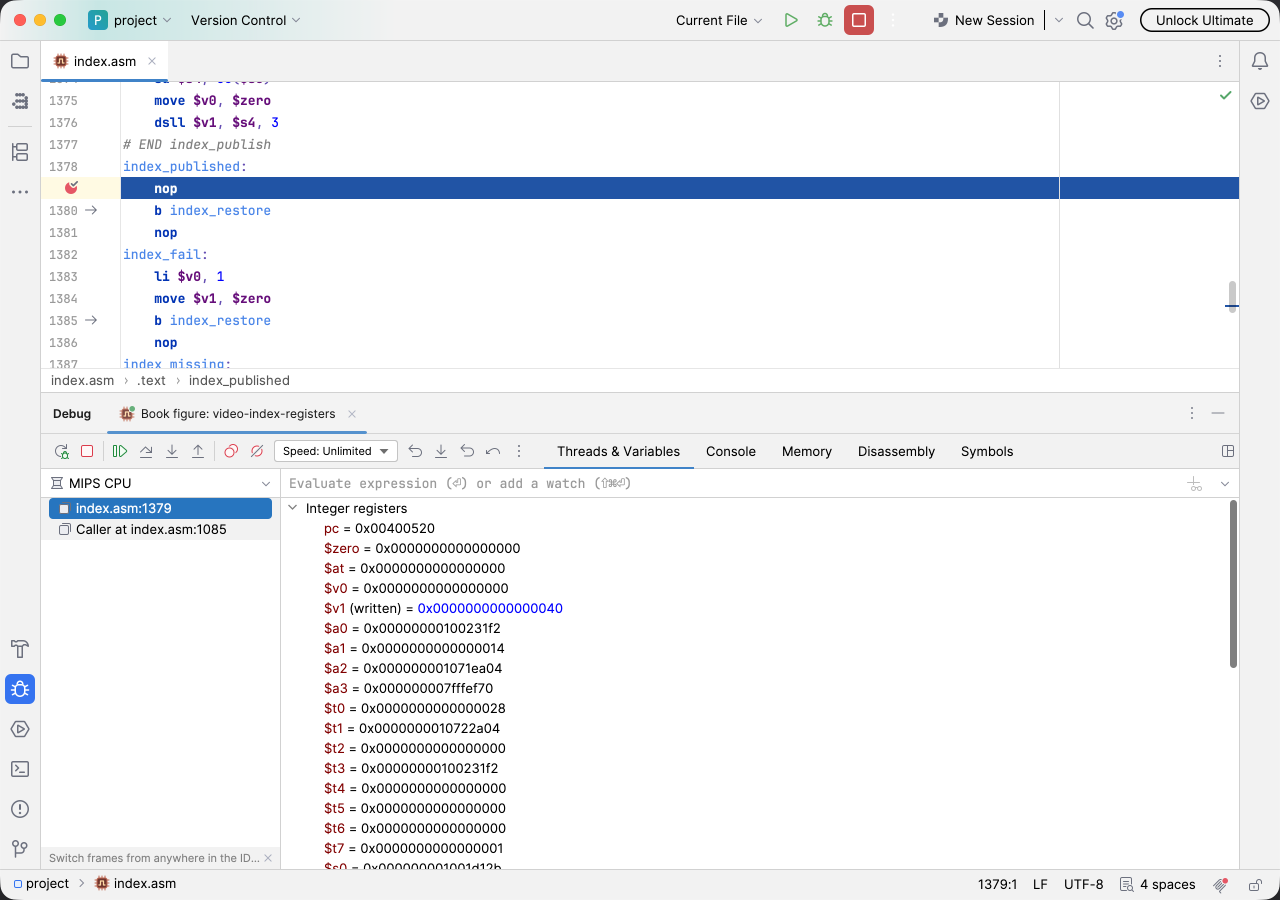
\includegraphics[width=0.52\linewidth,artifact,trim={\MARSindexreturnsLeft{} \MARSindexreturnsBottom{} \MARSindexreturnsRight{} \MARSindexreturnsTop{}},clip]{book/captures/034-lossless-video/video-index-publication/registers.png}};
\begin{scope}[shift={(returns.south west)},x={($(returns.south east)-(returns.south west)$)},y={($(returns.north west)-(returns.south west)$)}]
\draw[black,line width=0.7pt] (0.023437500,0.000000000) rectangle (0.976562500,1.000000000);
\node[draw=black,fill=white,circle,inner sep=1.5pt,font=\footnotesize] at ($(0.023437500,1.000000000)+(-3mm,0)$) {4};
\end{scope}
\end{tikzpicture}
\par\smallskip
\begin{minipage}{\linewidth}
\small
\begin{enumerate}
\item Publication is complete; the checkpoint \texttt{nop} has not executed.
\item Read each offset as a low/high pair of 32-bit words in this little-endian run. The first two and last two \texttt{a5a5a5a5} words retain the supplied pattern outside the eight active entries.
\item The first pair retains scratch capacity \texttt{0x4000}. The following pairs publish count eight, period four, duration forty, file bytes \texttt{0x60db} and eight entries.
\item \texttt{\$v0} is zero; \texttt{\$v1} is \texttt{0x40}, the 64 bytes occupied by eight entries.
\end{enumerate}
\end{minipage}
\caption{An accepted eight-frame file at the index-publication checkpoint. Three Debug launches show the same source, input and suspension point.}
\label{fig:video-index-publication}
\end{figure}
